\begin{table}[t]
	\centering
	\caption{Noise and effective resolution measurements of the acquisition chain.}
	\label{tab:noise_measurements}
	
	\begin{subtable}[t]{0.49\textwidth}
		\centering
		\caption{Voltage noise evaluation.}
		\label{tab:voltage_noise}
		
		\footnotesize
		\renewcommand{\arraystretch}{1.5}
		
		\resizebox{\linewidth}{!}{
			\begin{tabular}{c|c|c|c|c}
				\toprule
				$\mathrm{OSR}$ & $\measure{\mathrm{ENOB}}{[bit]}$ & $\measure{\mathrm{LSB}_{eff}}{[mV]}$ & $\measure{\sigma_m}{[mVrms]}$ & $\measure{V_{off}}{[mV]}$ \\
				\midrule
				
				\multicolumn{5}{c}{\textit{Channel A}} \\
				\midrule
				$128$ & $13.5$ & $36.6$ & $10.60$ & $-196.70$\\
				$256$ & $13.9$ & $28.2$ & $8.15$ & $-196.89$\\
				$512$ & $14.1$ & $23.8$ & $6.87$ & $-196.40$\\
				$1024$ & $14.4$ & $20.2$ & $5.82$ & $-195.90$\\
				
				\midrule
				
				\multicolumn{5}{c}{\textit{Channel B}} \\
				\midrule
				$128$ & $13.5$ & $36.6$ & $10.60$ & $-210.00$\\
				$256$ & $13.8$ & $28.8$ & $8.33$ & $-211.71$\\
				$512$ & $14.1$ & $24.3$ & $7.02$ & $-211.90$\\
				$1024$ & $14.2$ & $21.8$ & $6.28$ & $-212.00$\\
				
				\bottomrule
			\end{tabular}
		}
	\end{subtable}
	
	\vspace{0.5cm}
	
	\begin{subtable}[t]{0.49\textwidth}
		\centering
		\caption{Current noise evaluation.}
		\label{tab:current_noise}
		
		\footnotesize
		\renewcommand{\arraystretch}{1.5}
		\resizebox{\linewidth}{!}{
			\begin{tabular}{c|c|c|c|c}
				\toprule
				$\measure{\mathrm{FSR}}{[mA]}$ & $\measure{\mathrm{ENOB}}{[bit]}$ & $\measure{\mathrm{LSB}_{eff}}{[\mu A]}$ & $\measure{\sigma_m}{[\mu Arms]}$ & $\measure{I_{off}}{[uA]}$ \\
				\midrule
				
				\multicolumn{5}{c}{\textit{Channel A}} \\
				\midrule
				$\pm1.31$ & 13.8 & $0.19$ & $0.05$ & $0.20$\\
				$\pm13.06$ & 14.1 & $1.48$ & $0.43$ & $1.89$\\
				$\pm127.99$ & 14.1 & $14.3$ & $4.12$ & $18.87$\\
				$\pm1281.23$ & 14.0 & $159.08$ & $45.92$ & $177.9$\\
				
				\midrule
				
				\multicolumn{5}{c}{\textit{Channel B}} \\
				\midrule
				$\pm1.31$ & 13.6 & $0.21$ & $0.06$ & $0.03$\\
				$\pm13.06$ & 14.1 & $1.54$ & $0.44$ & $0.01$\\
				$\pm127.99$ & 14.3 & $12.67$ & $3.66$ & $0.34$\\
				$\pm1281.23$ & 13.7 & $188.92$ & $54.54$ & $-6.31$\\
				
				\bottomrule
			\end{tabular}
		}
	\end{subtable}
\end{table}

To assess the functionality and performance of the proposed system, a comprehensive set of tests was conducted. The initial test campaign was aimed at verifying compliance with the requirements listed in Table~\ref{tab:meas_ranges}, whereas subsequent tests were performed to evaluate the system performance and characterize its operational behavior. During this stage, a dedicated test application was used in place of the MARTe2 framework in order to isolate the hardware performance and simplify the validation procedure. In addition, all data analysis and parameter extraction were performed offline after the acquisition stage.


\subsection{Noise, Resolution \& Offsets Evaluation} \label{subsecVA}

\begin{figure*}[t]
	\centering
	\subfloat[Floating potential measurement in FP configuration]{
		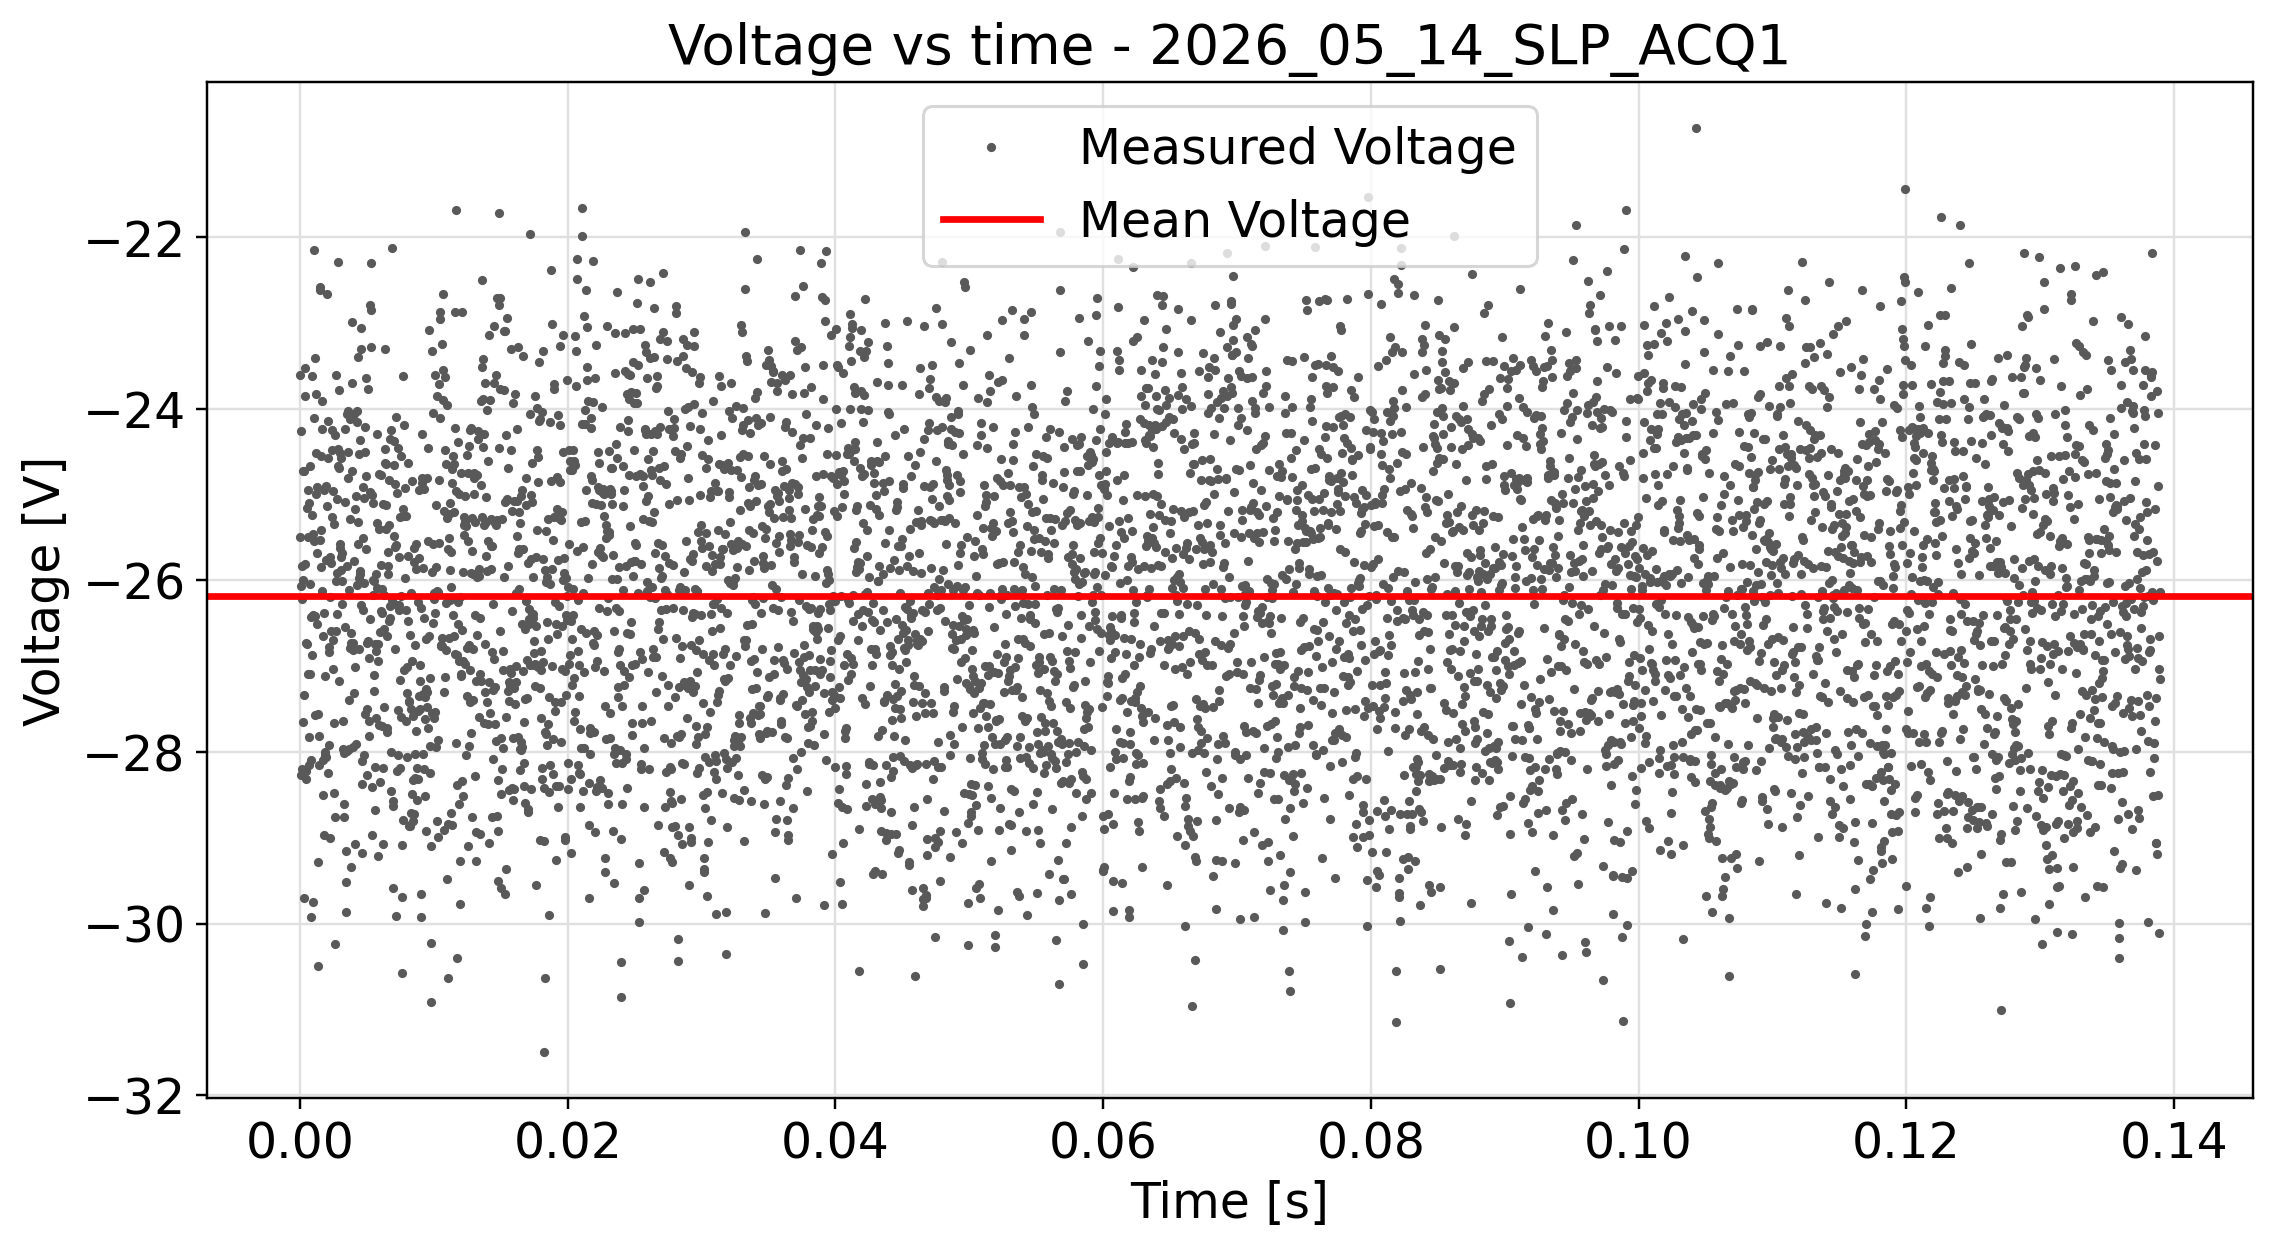
\includegraphics[width=3.4in]{2026_05_14_SLP_ACQ1_voltage_time}
		\label{fig5a}
	}
	\hfill
	\subfloat[SLP characteristic. The plot shows the four-parameter fit (red line) and the plasma parameters extracted from the measurement.]{
		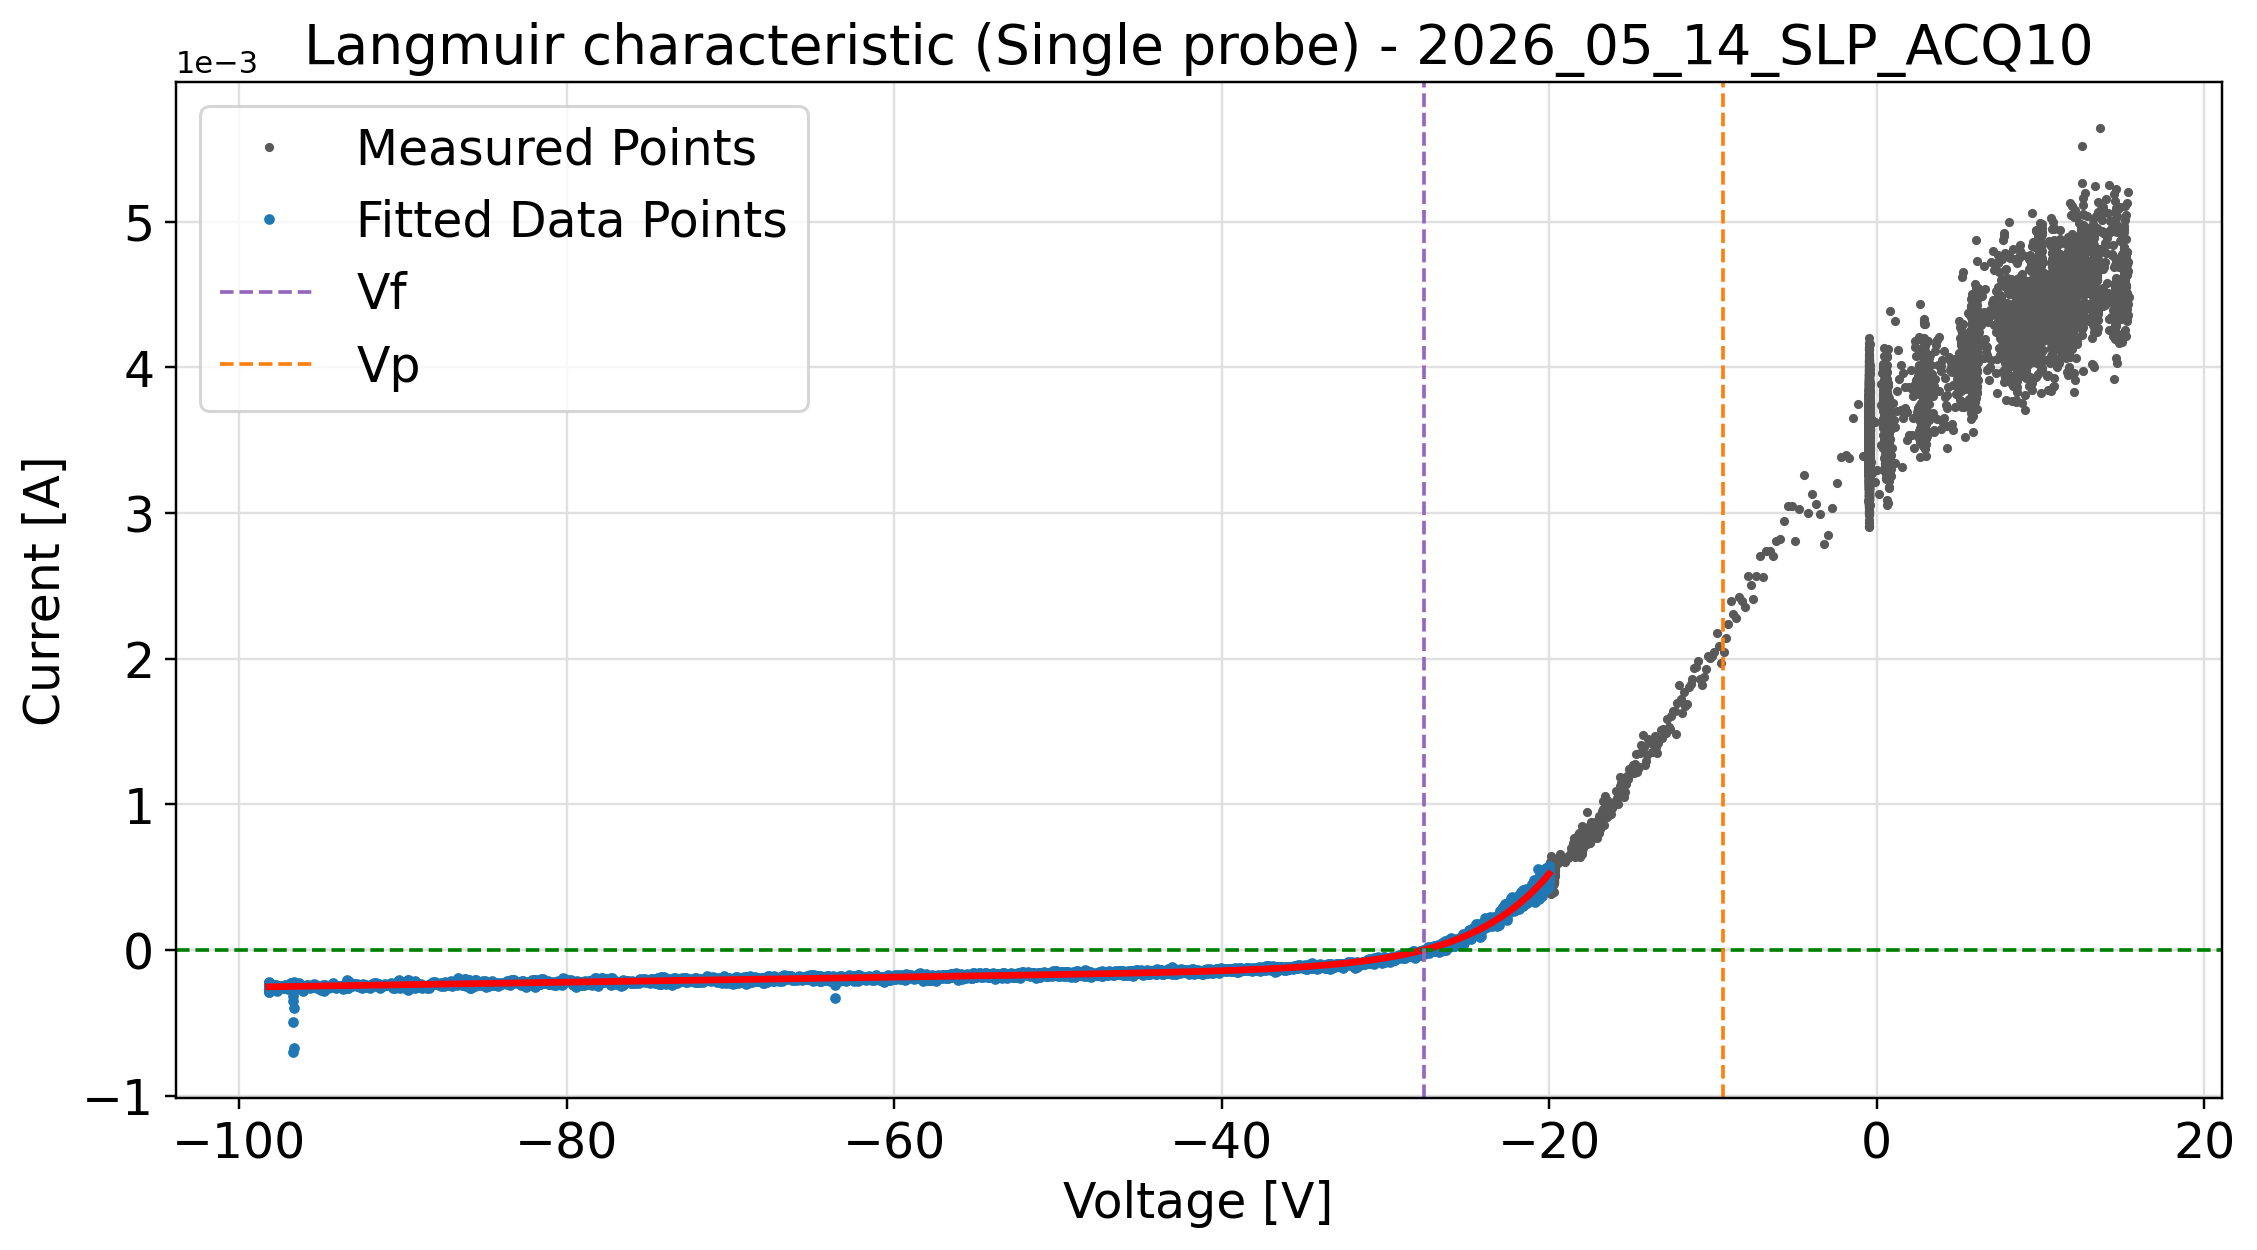
\includegraphics[width=3.4in]{2026_05_14_SLP_ACQ10_fits}
		\label{fig5b}
	}
	
	\caption{Representative floating-potential acquisition and SLP characteristic obtained during EPICA evaluation.}
	\label{fig5}
\end{figure*}

Several parameters were evaluated to quantify the performance of the acquisition chain. For both the voltage and current acquisition channels, the ENOB, the residual rms noise $\sigma_m$, the effective quantization step $\mathrm{LSB}_{eff}$, and the mean value $\mu_m$, representing the channel offset, were measured. The parameter $\sigma_m$ represents the residual noise floor of the acquisition chain, whereas $\mathrm{LSB}_{eff}$ corresponds to the effective resolution associated with the measured noise level. The ENOB can be estimated from the measured rms noise by considering the quantization error of an ideal analog-to-digital converter. The quantization error is uniformly distributed within the interval $\left[-\mathrm{LSB}_{eff}/2, +\mathrm{LSB}_{eff}/2\right]$ therefore, its standard deviation is
\begin{equation}
	\sigma_q = \frac{\mathrm{LSB}_{eff}}{\sqrt{12}}.
	\label{eq:ENOB1}
\end{equation}
By equating the measured rms noise $\sigma_m$ to the equivalent quantization noise, the effective resolution can be expressed as
\begin{equation}
	\mathrm{ENOB} = \log_2\left(\frac{\mathrm{FSR}}{\sigma_{m}\sqrt{12}}\right),
	\label{eq:ENOB2}
\end{equation}
where FSR denotes the full-scale range of the acquisition channel, LSB the nominal Least Significant Bit, and $\mathrm{LSB}_{eff}$ the effective quantization step corresponding to the measured noise floor. The corresponding nominal and effective quantization steps are
\begin{equation}
	\mathrm{LSB} = \frac{\mathrm{FSR}}{2^{16}}, \qquad \mathrm{LSB}_{eff} = \frac{\mathrm{FSR}}{2^{\mathrm{ENOB}}}.
	\label{eq:ENOB3}
\end{equation}

The voltage noise performance was evaluated with the integrated BPS disconnected from the probe circuitry by configuring both channels in FP mode. By configuring the system in FP mode, noise contributions from the BPS are excluded from the measurement, allowing the performance of the analog front-end and ADC acquisition chain to be evaluated independently. The inputs were subsequently short-circuited in order to eliminate external noise sources. ENOB and effective resolution values, computed using (\ref{eq:ENOB1}) and (\ref{eq:ENOB3}), are summarized in Table~\ref{tab:voltage_noise}. The voltage acquisition chain has a nominal full-scale range of $\mathrm{FSR}=\measure{423.03}{V}$, corresponding to a nominal quantization step of $\mathrm{LSB}=\measure{6.455}{mV}$, which is equal for each voltage channel. The nominal FSR differs from the value reported in Table~\ref{tab:meas_ranges} due to the voltage-divider ratio adopted in the acquisition chain. This design choice was made to preserve the capability of measuring higher voltages when external bias supplies are used in place of the integrated BPS. Table \ref{tab:voltage_noise} summarizes the measured noise and effective resolution values.

Current measurement validation was performed by configuring the probe module in the SLP operating mode and applying an external fixed bias voltage for each current FSR. This approach was adopted to ensure that noise contributions associated with the integrated BPS were excluded from the evaluation of the acquisition chain performance. During these tests, the acquisition frequency was fixed at $F_s=\measure{78.125}{kHz}$.

Evaluation of the offsets ($V_{off}$ and $I_{off}$) related to each channel and FSR was carried out applying the same procedure of the current noise evaluation, physically detaching the integrated BPS and short circuiting the BPS rails of the analog front-end and the inputs.



\subsection{Probe Characteristic} \label{subsecVB}

Characterization of the overall system behavior was carried out using a dedicated vacuum chamber capable of generating low-temperature plasmas. Plasma operating conditions were controlled through adjustments of the gas pressure and electrode bias voltage, thereby enabling the generation of different plasma regimes. 

Plasma parameters were estimated by fitting the acquired I-V characteristics using the four-parameter model
\begin{equation}
	I(V)=I_s\left[1+R(V-V_f)\right] \left(e^{\frac{V-V_f}{T_e}}-1\right),
	\label{eq:model_slp}
\end{equation}
where $T_e$ is the electron temperature, $I_s$ the ion saturation current, $V_f$ the floating potential, and $R$ a linear correction factor accounting for deviations from the ideal ion saturation regime. Once the fitting parameters $(T_e, I_s, V_f, \mathrm{R})$ were obtained, $N_e$ and $V_p$ were estimated from the fitted floating potential and electron temperature according to the classical Langmuir probe theory \cite{Chen}. A preliminary acquisition was performed in the FP configuration to determine the probe floating potential. The corresponding measurement is shown in Fig.~\ref{fig5a}. Unlike the noise characterization tests described in Section~\ref{subsecVA}, the measured fluctuations in this case include contributions from both the acquisition chain and the plasma itself. Consequently, the observed noise level is significantly higher than the intrinsic noise floor of the instrumentation. The FP measurement yielded a mean floating potential of $V_f=\measure{-26.2}{V}$ and an RMS fluctuation level of $\sigma_m=\measure{1.81}{Vrms}$. Subsequently, the system was operated in the SLP configuration to acquire the complete I-V characteristic. A representative characteristic obtained from a helium plasma is shown in Fig.~\ref{fig5b}. The corresponding plasma parameters are reported in Table \ref{tab:SLP}.

Whereas the FP and SLP configurations were successfully tested using the plasma source, validation of the DLP configuration was limited by the inability to place two probes in regions characterized by sufficiently uniform plasma conditions. Therefore, a dummy load comprising a resistor and two anti-series Zener diodes was connected to the probe module. This setup was used to verify the correct operation of the front-end switching network and the associated acquisition circuitry under DLP conditions. The resulting I-V characteristic is shown in Fig.~\ref{fig6}

\begin{figure}[t]
	\centering
	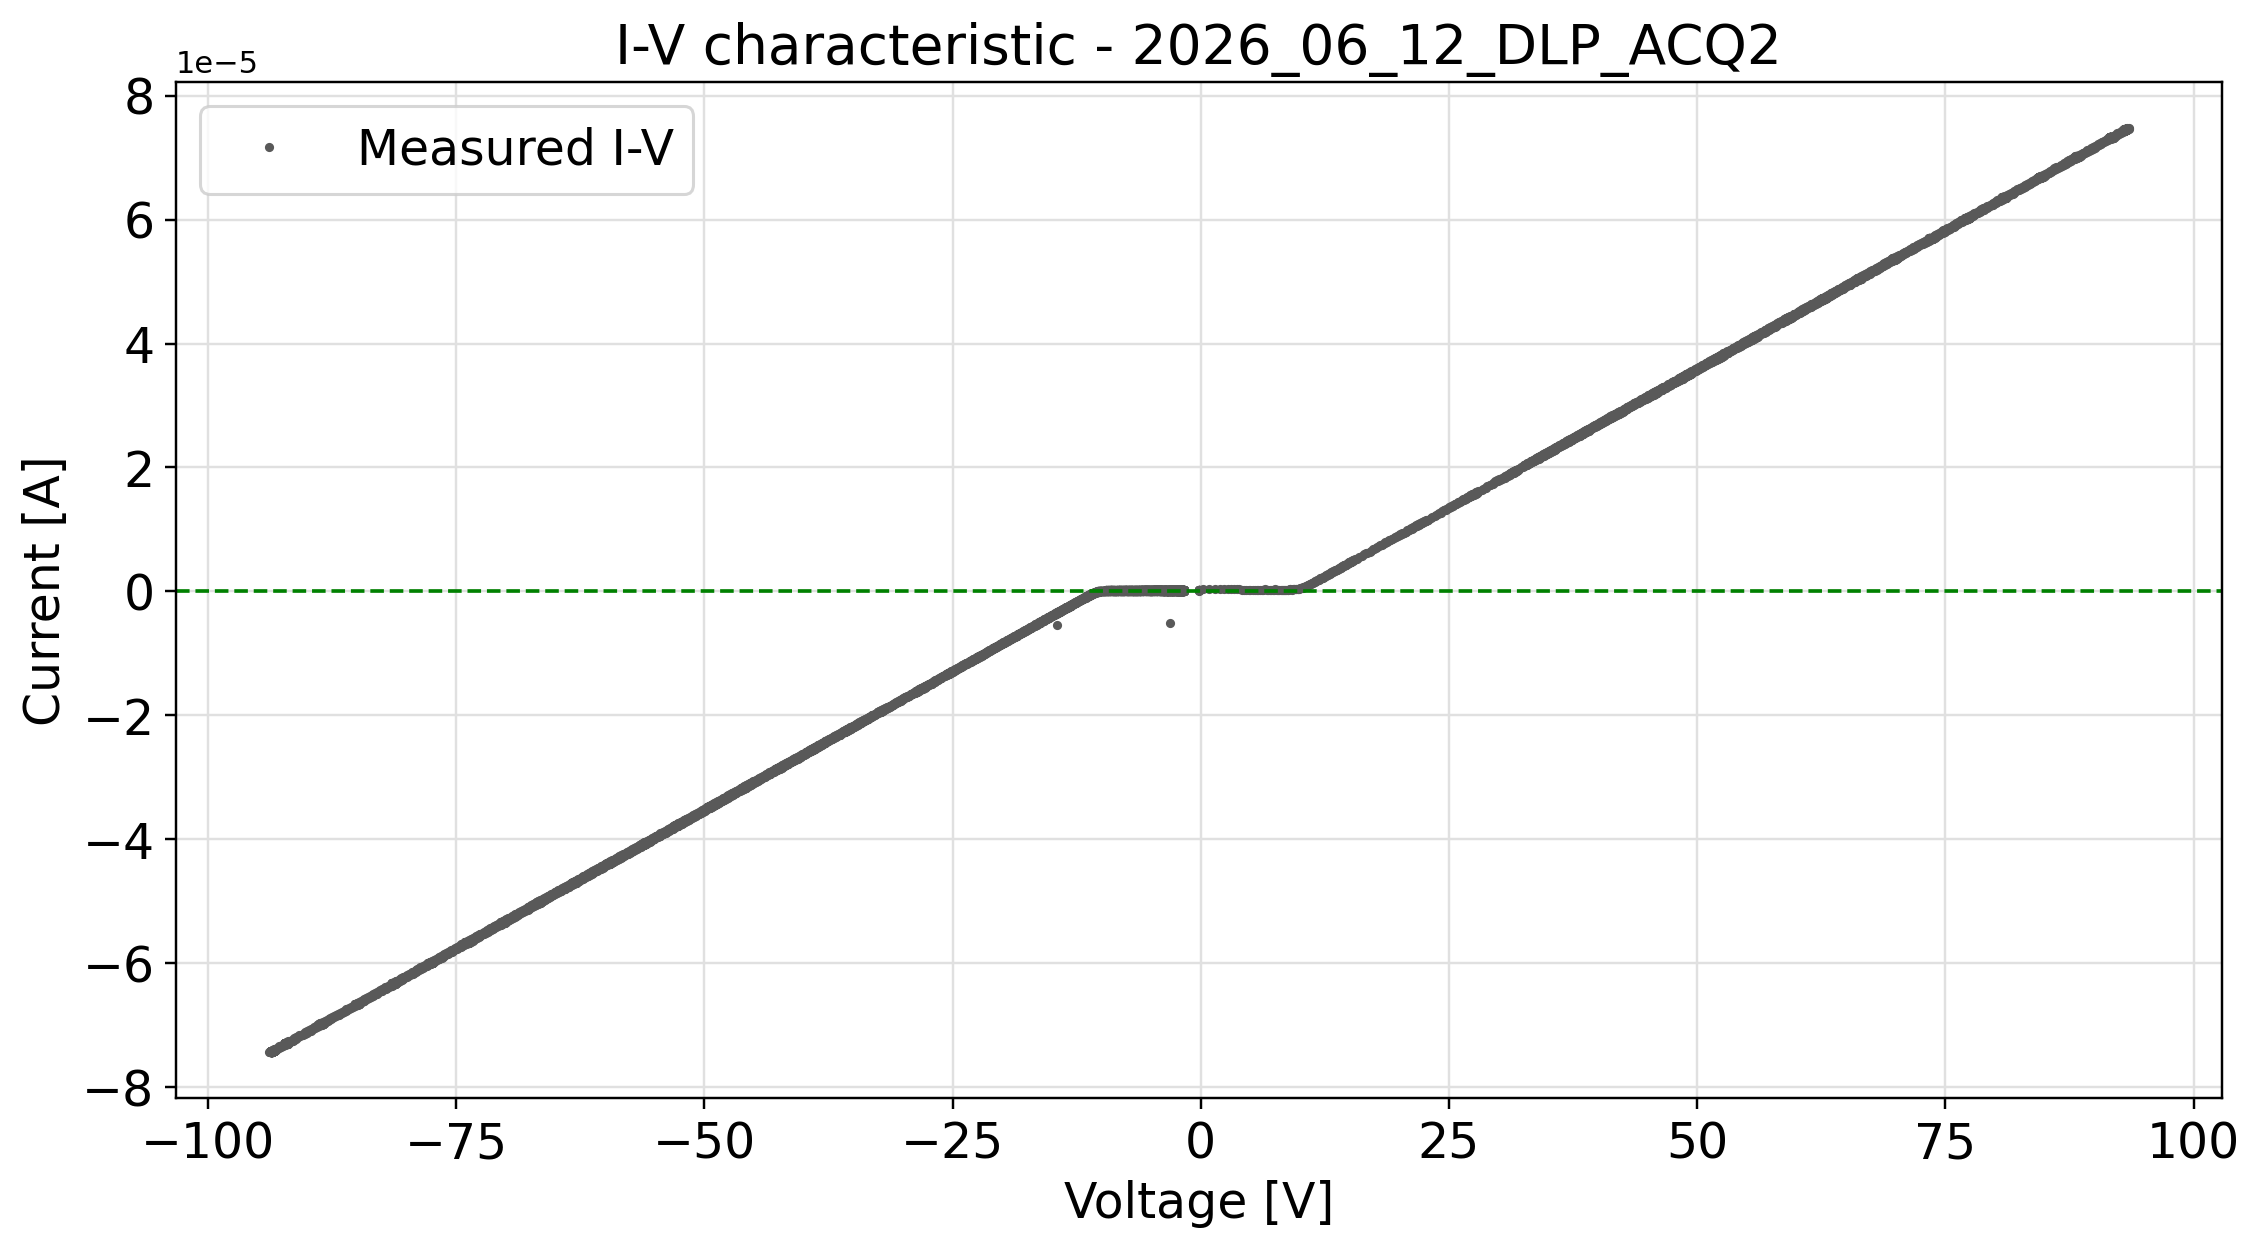
\includegraphics[width=3.4in]{2026_06_12_DLP_ACQ2_i-v}
	\caption{Functional verification of the DLP configuration using a dummy load composed of anti-series Zener diodes. Acquisition performed at $F_s = \measure{78.125}{kHz}$ and $\mathrm{FSR} = \measure{\pm1}{mA}$.}
	\label{fig6}
\end{figure}

\begin{table}[t]
	\centering
	\footnotesize
	\renewcommand{\arraystretch}{1.5}
	\caption{Plasma parameters extrapolated from the SLP characteristics.}
	\label{tab:SLP}
	
	\begin{tabular}{c|c|c|c|c}
		\toprule
		$\measure{T_e}{[eV]}$ & $\measure{I_s}{[A]}$ & $\measure{V_f}{[V]}$ & $\measure{V_p}{[V]}$ & $\measure{N_e}{[m^{-3}]}$\\
		\midrule
		$4.53$ & $1.31\cdot10^{-4}$ & $-27.7$ & $-9.39$ & $7.82\cdot10^{16}$\\
		\bottomrule
	\end{tabular}
	
\end{table}
